\documentclass[12pt,a4paper]{article}

% ── Packages ──────────────────────────────────────────────────────────────────
\usepackage[utf8]{inputenc}
\usepackage[T1]{fontenc}
\usepackage[french]{babel}
\usepackage{geometry}
\geometry{margin=2.5cm}
\setlength{\headheight}{15pt}

\usepackage{graphicx}
\usepackage{hyperref}
\hypersetup{colorlinks=true, linkcolor=blue, urlcolor=blue, citecolor=blue}
\usepackage{booktabs}
\usepackage{float}
\usepackage{amsmath}
\usepackage{amssymb}
\usepackage{enumitem}
\usepackage{listings}
\usepackage{xcolor}
\usepackage{fancyhdr}
\usepackage{caption}

% ── Code style ────────────────────────────────────────────────────────
\lstset{
  basicstyle=\ttfamily\small,
  keywordstyle=\color{blue}\bfseries,
  stringstyle=\color{red},
  commentstyle=\color{green!60!black}\itshape,
  backgroundcolor=\color{gray!5},
  frame=single,
  rulecolor=\color{gray!40},
  breaklines=true,
  tabsize=4,
  captionpos=b,
  showstringspaces=false
}

% ── Header / Footer ────────────────────────────────────────────────────────────
\pagestyle{fancy}
\fancyhf{}
\rhead{Projet IA - Jeu d'Escampe}
\lhead{Rapport Final}
\cfoot{\thepage}

% ── Title ──────────────────────────────────────────────────────────────────────
\title{
  \Large \textbf{Conception et Implémentation d'une Intelligence Artificielle pour le Jeu d'Escampe}\\[0.4em]
}
\author{
  Mathieu \textsc{Waharte} \and Raphaël \textsc{Binda}
}
\date{Mai 2026}

\begin{document}

\maketitle
% \thispagestyle{fancy}

\begin{abstract}
Ce rapport détaille la conception et la mise en oeuvre d'une IA capable de jouer au jeu d'Escampe avec contraintes de temps total. Nous y présentons nos choix d'implantation, notamment les structures de données optimisées (Bitboards), les algorithmes de recherche (Negamax avec élagage Alpha-Beta, Iterative Deepening) ainsi que la fonction d'évaluation heuristique développée pour modéliser la complexité topologique du plateau. Nous abordons également les stratégies de placement initial, la gestion dynamique du temps d'exécution, et fournissons une analyse des performances validées par des tests rigoureux.
\end{abstract}

\vspace{0.5em}
\noindent\rule{\linewidth}{0.4pt}
\tableofcontents
\vspace{1em}



\newpage
\section{Introduction}
Dans le cadre de ce projet, l'objectif principal est de développer une Intelligence Artificielle capable de conduire de façon autonome une partie d'Escampe en temps limité (300s à 900s par joueur). L'agent doit communiquer avec un arbitre validant les coups et garantissant le respect des contraintes temporelles.
Le jeu d'Escampe se caractérise par des règles de déplacement atypiques (dépendance à la bande ciblée par l'adversaire) et une asymétrie de la topologie du plateau. Ces spécificités requièrent des choix algorithmiques pointus, s'écartant parfois des implémentations classiques des jeux à information parfaite.


\subsection{Fin de Partie}
Une partie se termine dès qu'un joueur capture la licorne adverse en y déplaçant un paladin. Aucun score partiel n'existe, seule la capture compte. Pour les agents, il convient d'ajouter un mécanisme de détection de répétition de position afin d'éviter les boucles infinies.


\subsection{Analyse de la Complexité}
\paragraph{Facteur de branchement.}
Chaque pièce peut se déplacer dans au plus 4 directions lors de son premier saut, puis 3 directions pour les suivants (sans revenir sur ses pas), avec jusqu'à 3 sauts selon sa bande. Dans le pire des cas, avec 6 pièces :
\[
b_{\max} = 6 \times (4 + 2 \times 3) = 60 \text{ coups légaux par tour.}
\]
En pratique, la contrainte de bande, les bords du plateau et les blocages ramènent ce facteur à 15-25 coups légaux en position typique de milieu de partie, ce qui justifie l'emploi d'un élagage Alpha-Beta agressif.

\paragraph{Majorant du nombre d'états.}
En modélisant un état de jeu par les positions des 12 pièces parmi 36 cases et la bande imposée par le dernier coup (4 valeurs), on obtient :
\[
\mathcal{M} = \binom{36}{1}\binom{35}{5}\binom{30}{1}\binom{29}{5} \times 4 = \frac{36!}{(5!)^2\,(36-12)!} \times 4 \approx 1{,}67 \times 10^{14}
\]
états distincts. Ce chiffre confirme que toute exploration exhaustive est impossible et que les heuristiques et l'élagage sont indispensables.

\paragraph{Sources de difficulté.}
Au-delà de la complexité combinatoire, les principales difficultés algorithmiques sont : (i) la contrainte de bande qui conditionne les pièces jouables au tour suivant, créant des effets de tempo et de forçage, (ii) l'absence de simplification rapide (pas de capture de pions), qui allonge les séquences tactiques et (iii) l'importance du placement initial qui engendre une forte variabilité de départ.





\section{Choix d'Implantation et Structures de Données}
Afin de garantir des performances optimales lors de l'exploration de l'arbre de jeu, les structures de données sous-jacentes doivent permettre une génération de coups et une évaluation d'états extrêmement rapides.


\subsection{Structure Générale du Projet}
Le code source est structuré en plusieurs packages modulaires favorisant la séparation des responsabilités et le découplage des composants :
\begin{itemize}
    \item \textbf{Package \texttt{interfaces}} : Définit les contrats essentiels pour l'ensemble du projet : \texttt{IJoueur} (contrat requis par l'arbitre), \texttt{IBoard} (abstraction du plateau), \texttt{IMove} (représentation générique d'un coup), \texttt{IRole} (rôle du joueur), et \texttt{IHeuristic} (contrat pour les fonctions d'évaluation heuristique).
    \item \textbf{Package \texttt{game}} : Contient les implémentations physiques et conceptuelles du jeu. \texttt{EscampeBoard} modélise l'état et les transitions du plateau par le biais de Bitboards, \texttt{EscampeMove} représente un déplacement (coordonnées de départ, intermédiaires, d'arrivée et contrainte de bande), et \texttt{EscampeAIPlayer} implémente le joueur autonome, gérant l'approfondissement itératif et la délégation de la recherche.
    \item \textbf{Package \texttt{algorithms}} : Regroupe la logique de décision. Il se subdivise en :
        \begin{itemize}
            \item \texttt{algorithms.search} : Implémente les algorithmes de recherche (\texttt{NegamaxKH}, \texttt{AlphaBetaKH}) ainsi que la classe d'ordonnancement \texttt{MoveOrderer} (Killer Moves + History Heuristic).
            \item \texttt{algorithms.evaluation} : Contient la fonction d'évaluation linéaire (\texttt{Heuristic}, \texttt{HeuristicConfig}).
            \item \texttt{Opening} : Gère la bibliothèque de départ (ouvertures pré-calculées).
            \item \texttt{TimeManager} : Calcule dynamiquement le budget temporel restant.
        \end{itemize}
    \item \textbf{Package \texttt{model}} : Contient la classe \texttt{DataExport} chargée de sérialiser et d'exporter les états de jeu joués au format JSON. Ces données d'apprentissage alimentent le pipeline d'entraînement Python du modèle de réseau de neurones BandDPER.
    \item \textbf{Package \texttt{ranking}} : Dédié à la validation et aux tournois comparatifs. Il contient \texttt{TournamentRunner} (simulation locale en parallèle), \texttt{AIRankingSystem} (suivi des classements Elo et tests statistiques SPRT) et \texttt{SimplexTuner} (implémentation de l'optimisation Simplex pour l'heuristique).
    \item \textbf{Package \texttt{io}} : Gère les interfaces d'exécution. \texttt{ClientJeu} assure la communication réseau TCP avec le serveur de l'arbitre, \texttt{Solo} permet de lancer une partie locale directe entre deux bots pour le débogage et \texttt{Applet} fournit le rendu graphique visuel.
\end{itemize}


\subsection{Représentation du Plateau (Bitboards hybrides)}
Nous avons opté pour une représentation du plateau basée sur un tableau de \texttt{char} de 36 cases ainsi que des \textit{Bitboards}~\cite{cp_bitboards}. Les bitboards sont utilisés pour calculer rapidement les coups légaux, les collisions et les menaces, tandis que le tableau de caractères sert au stockage de l'état de manière simplifiée.
\begin{itemize}
    \item Les opérations de manipulation de pièces (génération des coups, détection de collisions) se réduisent à des opérations bit à bit (ET, OU, décalages), exécutées en un seul cycle d'horloge.
    \item Cette approche permet d'éliminer les itérations coûteuses sur des tableaux multidimensionnels et minimise la création d'objets, limitant ainsi la pression sur le \textit{Garbage Collector}.
\end{itemize}


\subsection{Optimisations d'Implémentation}
Plusieurs choix techniques ont été faits pour maximiser le nombre de noeuds explorés par seconde :
\begin{itemize}
  \item \textbf{Stratégie Make-Unmake} (annulation de coup) : plutôt que de cloner le plateau à chaque noeud de l'arbre, les coups sont joués sur le plateau courant puis défaits après évaluation (\texttt{board.undo(move, role)}). Cette approche élimine toute allocation mémoire dans la boucle de recherche et réduit la pression sur le \textit{Garbage Collector}.
    \item \textbf{Suppression des appels \texttt{instanceof}} lors de la génération des coups via des méthodes dédiées par type de pièce, évitant le coût du dispatch polymorphique à chaque noeud.
    \item \textbf{Pré-allocation des structures} : les tableaux de positions de pièces (paladins, licornes) et les masques de Bitboards sont alloués une seule fois. Le tri de la liste des coups est réalisé en place (\textit{insertion sort} sans copie, cf. section~\ref{sec-move-ordering}).
    \item \textbf{Table de transposition (Zobrist Hashing)~\cite{cp_zobrist}} : le schéma d'encodage (XOR de valeurs aléatoires 64 bits par pièce et par case, entrées de table stockant profondeur, type de noeud, score et meilleur coup) a été entièrement conçu mais non intégré dans la version finale par contrainte de temps. Elle constitue l'optimisation la plus prometteuse pour des versions futures, pouvant notamment permettre la détection de répétition de position.
\end{itemize}






\section{Algorithmes de Recherche du Meilleur Coup}
La recherche du meilleur coup repose sur la théorie de la recherche adversarielle pour les jeux à somme nulle.

\subsection{Negamax et Élagage Alpha-Beta}
Nous avons implémenté l'algorithme Negamax (une variante élégante du Minimax) couplé à un élagage Alpha-Beta~\cite{cp_alphabeta, knuth1975}. Cette approche unifie l'évaluation pour les deux joueurs, réduisant ainsi la complexité du code. L'élagage Alpha-Beta permet de réduire drastiquement le facteur de branchement effectif de l'arbre de recherche en ignorant les branches dont il est prouvé qu'elles sont sous-optimales.
Avant cela, nous avons expérimenté avec le Minimax classique puis l'Alpha-Beta simple, mais la version Negamax fut la plus performante. Un problème rencontré avec Negamax concernait l'utilisation des valeurs \texttt{Integer.MIN\_VALUE} et \texttt{Integer.MAX\_VALUE} pour $\alpha$ et $\beta$ : lors de l'inversion de signe, cela causait des dépassements d'entier (integer overflow). Nous avons résolu ce problème en utilisant des valeurs de garde légèrement inférieures à ces extrêmes.


\subsection{Approfondissement Itératif (Iterative Deepening)}
Pour exploiter au mieux le temps imparti, la recherche est structurée autour d'un approfondissement itératif~\cite{cp_iterative_deepening}. L'algorithme explore l'arbre progressivement : à profondeur 1, puis 2, puis 3, et ainsi de suite jusqu'à la limite \texttt{depthMax}. 
À chaque nouvelle itération de profondeur, le temps écoulé est vérifié via notre limite de calcul logicielle (\textit{Soft Bound}). Si cette limite est atteinte en cours d'itération, l'algorithme abandonne l'itération incomplète en cours et renvoie immédiatement le meilleur coup validé lors de la \textit{dernière itération complétée}. Ce mécanisme garantit qu'un coup fiable et profondément évalué est toujours disponible sans risque de dépassement.

Une amélioration envisagée mais non intégrée dans les délais du projet est l'utilisation de fenêtres d'aspiration (\textit{Aspiration Windows}) : au lieu de relancer chaque itération avec une fenêtre pleine ($\alpha = -\infty$, $\beta = +\infty$), on initialiserait $\alpha$ et $\beta$ autour du score de la profondeur précédente (par exemple à $\pm 50$). En cas d'échec (\textit{fail-low} ou \textit{fail-high}), la fenêtre serait élargie et la recherche relancée. Cette technique peut réduire significativement le nombre de noeuds à explorer lorsque le score est stable entre deux profondeurs successives.


\subsection{Ordonnancement des Coups et Élagage Sélectif}
\label{sec-move-ordering}
L'efficacité de l'élagage Alpha-Beta dépend directement de la qualité de l'ordonnancement des coups~\cite{cp_move_ordering} : dans le cas idéal, chaque noeud MIN ne considère qu'un seul coup (l'élagage est immédiat). Les deux techniques suivantes, encapsulées dans la classe \texttt{MoveOrderer}, ont été implémentées.

\paragraph{Killer Heuristic~\cite{cp_killer}.}
À chaque profondeur de l'arbre, on maintient un tableau de 2 \textit{killer moves}, qui sont des coups ayant provoqué une coupure Beta dans un noeud frère à la même profondeur. Ces coups sont essayés en priorité (score fixe \texttt{KILLER\_SCORE} = 900\,000), car il est probable qu'ils causent à nouveau une coupure dans le noeud courant. L'enregistrement suit une file FIFO à 2 slots : le nouveau killer déplace le premier, qui passe en second slot, préservant ainsi un \textit{backup} fiable.

\paragraph{History Heuristic.}
Un tableau plat \texttt{historyTable[36 $\times$ 36]} indexé par l'encodage du coup (case de départ $\times$ 36 + case d'arrivée, soit 1\,296 entrées sur un plateau 6$\times$6) accumule un score à chaque coupure Beta, pondéré par $\text{profondeur}^2$. Ce poids favorise les coupures profondes, statistiquement plus significatives. Les coups historiquement les plus coupants remontent naturellement en tête de liste sans aucun coût d'allocation.

\paragraph{Tri in-place par insertion.}
L'ordonnancement combine les deux scores (killer prioritaire, puis historique) et trie la liste de coups par insertion directement dans l'objet \texttt{ArrayList} renvoyé par \texttt{possibleMoves()}. Le tri par insertion est optimal pour de petites listes, le nombre de coups légaux en Escampe ne dépasse généralement pas 30.

\paragraph{Techniques non implémentées.}
Le \textit{Transposition Table Move} (essai en tête de liste du meilleur coup issu de la table de transposition~\cite{cp_killer}), le \textit{Null-move Pruning}~\cite{cp_nullmove} et le \textit{Late Move Reduction}~\cite{cp_lmr} ont été identifiés comme des améliorations à fort potentiel, mais n'ont pas été intégrés dans les délais du projet. Ils constituent des priorités pour des versions ultérieures.





\section{Fonction d'Évaluation (Heuristiques)}
L'évaluation des feuilles de l'arbre de recherche se doit d'être précise tout en demeurant très rapide à calculer. Notre heuristique est une combinaison linéaire de plusieurs signaux topologiques, suivant l'approche classique formalisée par Shannon~\cite{shannon1950}.


\subsection{Heuristiques Implémentées et Testées}
La fonction d'évaluation s'articule autour des métriques suivantes :
\begin{enumerate}
    \item \textbf{Distances d'Attaque et de Défense} : Calcul de la distance de Manhattan entre les Paladins et les Licornes adverses. Plus les attaquants sont proches, meilleur est le score. L'heuristique pénalise la proximité des Paladins adverses à notre Licorne. \textit{Note: une implémentation avancée utilisant une distance en nombre de sauts (BFS ply) intégrant la contrainte des bandes a également été modélisée mais s'est avérée néfaste en raison du temps de calcul supplémentaire.}
    \item \textbf{Échappatoire de la Licorne (Escapability)} : Compte direct du nombre de cases légales de fuite pour la Licorne de chaque joueur. Un adversaire avec peu d'échappatoires est considéré comme dominé positionnellement.
    \item \textbf{Contrôle des Bandes (Band Control)} : La contrainte du jeu force l'adversaire à partir d'une bande spécifique. Le positionnement de nos Paladins sur des cases de bande 1 (où l'adversaire n'a aucun choix) est théoriquement valorisé pour contraindre l'adversaire. Cette partie de l'heuristique a été mise en question par les tests du tournoi et des études d'ablation. Elle a été retirée car elle dégradait la performance.
    \item \textbf{Pression Temporelle et Mobilité} : Récompense accordée pour un nombre de coups légaux plus élevé, et forte pénalité lorsqu'un joueur est forcé de passer son tour en raison du mécanisme de contrainte.
\end{enumerate}

La formule d'évaluation générale modélisée pour une position est la suivante :
\begin{align*}
\mathcal{H} &= - w_{1} \cdot d^{\text{atk}}_{\min} - w_{2} \cdot d^{\text{atk}}_{\text{avg}} + w_{3} \cdot d^{\text{def}}_{\min} + w_{4} \cdot d^{\text{def}}_{\text{avg}} \\
            &+ w_{5} \cdot \mathcal{E}_{\text{us}} - w_{6} \cdot \mathcal{E}_{\text{opp}} + w_{7} \cdot (\mathcal{M}_{\text{us}} - \mathcal{M}_{\text{opp}}) - w_{8} \cdot \mathcal{MB}_{\text{us}} + w_{9} \cdot \mathcal{MB}_{\text{opp}} - \text{Passe}
\end{align*}
où :
\begin{itemize}
    \item $d^{\text{atk}}_{\min}$ et $d^{\text{atk}}_{\text{avg}}$ désignent respectivement la distance de Manhattan minimale et moyenne de nos paladins vers la licorne adverse (notés $w_1$ et $w_2$, de signe négatif car une distance faible favorise l'attaque).
    \item $d^{\text{def}}_{\min}$ et $d^{\text{def}}_{\text{avg}}$ désignent la distance minimale et moyenne des paladins adverses vers notre licorne (notés $w_3$ et $w_4$, de signe positif car l'éloignement favorise la défense).
    \item $\mathcal{E}_{\text{us}}$ est l'échappatoire de notre licorne (nombre de coups de fuite légaux, $w_5$).
    \item $\mathcal{E}_{\text{opp}}$ désigne l'échappatoire de la licorne adverse (nombre de coups de fuite légaux pour l'adversaire, $w_6$).
    \item $\mathcal{M}_{\text{us}}$ et $\mathcal{M}_{\text{opp}}$ désignent le nombre de coups légaux pour chaque joueur ($w_7$).
    \item $\mathcal{MB}_{\text{us}}$ et $\mathcal{MB}_{\text{opp}}$ représentent le nombre de liserés/bandes non couverts parmi les bandes 1, 2, et 3 (pénalité de $-w_8$ si nos pièces ne couvrent pas toutes les bandes, et bonus de $+w_9$ si l'adversaire a des bandes non couvertes).
    \item $\text{Passe}$ est une pénalité fixe de 500 points si le joueur actif est en situation de passe forcé, et un bonus de 100 points si l'adversaire doit passer.
\end{itemize}

Les poids configurés et testés au cours de nos différents runs de calibration sont détaillés dans le tableau~\ref{tab-heuristic-weights}.

\begin{table}[H]
\centering
\begin{tabular}{l c c c c}
\toprule
Poids & Default & SPSA-Tuned-Full & Simplex-Tuned-Full & Bayes-Tuned-Full \\
\midrule
$w_1$ (Min Atk Dist) & $10$ & $25$ & $41$ & $48$ \\
$w_2$ (Avg Atk Dist) & $2$ & $1$ & $0$ & $21$ \\
$w_3$ (Min Def Dist) & $5$ & $12$ & $5$ & $31$ \\
$w_4$ (Avg Def Dist) & $5$ & $0$ & $8$ & $38$ \\
$w_5$ (Licorne Escapability) & $50$ & $0$ & $114$ & $29$ \\
$w_6$ (Licorne Opp Trapped) & $30$ & $60$ & $69$ & $60$ \\
$w_7$ (Mobility / Legal Moves) & $10$ & $4$ & $13$ & $4$ \\
$w_8$ (Our Band Control) & $0$ & $0$ & $11$ & $-4$ \\
$w_9$ (Opp Band Control) & $0$ & $0$ & $-3$ & $-39$ \\
\bottomrule
\end{tabular}
\caption{Valeurs absolues des poids heuristiques selon les méthodes de calibration.}
\label{tab-heuristic-weights}
\end{table}


\paragraph{Calibration des poids par SPSA.}
Les neuf poids de la formule ont été calibrés empiriquement via l'algorithme SPSA (\textit{Simultaneous Perturbation Stochastic Approximation})~\cite{spall1998}, une méthode de descente de gradient stochastique particulièrement adaptée à l'optimisation de fonctions d'évaluation de jeux~\cite{cp_testing}. À chaque itération, les paramètres sont perturbés dans deux directions aléatoires ($\pm \delta$), deux parties sont jouées (une dans chaque configuration), et le gradient estimé est utilisé pour mettre à jour les poids. Le processus a été exécuté sur 50 itérations avec 16 paires de parties par itération (32 parties/itération), soit 1\,600 parties par run, en parallèle sur tous les coeurs disponibles.

Une étude d'ablation a révélé que le terme de contrôle des bandes ($w_8, w_9$) ne contribuait pas positivement : la configuration à 7 paramètres (termes de bande forcés à zéro) surpassait la configuration à 9 paramètres dans les tests croisés. La configuration finale retenue (\texttt{createAblated("bandcoverage")}) exclut donc ce terme. Ce résultat est contre-intuitif au vu de l'importance du mécanisme de bandes dans les règles du jeu, mais il est validé statistiquement. En revanche, les réglages Simplex et Bayes montrent que forcer l'adversaire sur des bandes non couvertes est une stratégie viable si elle est combinée à des poids d'attaque très agressifs.




\section{Exploration d'une Évaluation par Réseau de Neurones : BandDPER}
Bien que l'heuristique manuelle soit performante, les contraintes spatiales fortement non linéaires d'Escampe se prêtent bien à l'apprentissage automatique et il a été montré sur le jeu d'échecs~\cite{cp_nnue} ou de Go~\cite{alphazero} que les réseaux de neurones surpassent les méthodes traditionnelles.
Le modèle \textbf{BandDPER} (\textit{Band-Aware Dual-Perspective Equivariant ResNet}) a été conçu comme fonction d'évaluation alternative ou de support à l'ordonnancement des coups.


\subsection*{Choix du type de modèle}
\begin{table}[H]
\centering
\begin{tabular}{p{1.8cm} p{6.5cm} p{4.5cm}}
\toprule
Modèle & Notes & Recommandation \\
\midrule
MLP & Rapide, mais aucune notion spatiale ni raisonnement relationnel & À éviter \\
CNN & Exploite les motifs spatiaux locaux et l'équivariance par translation & Acceptable, légèrement surdimensionné \\
NNUE & Mises à jour incrémentales rapides, conception dual-perspective, activations ClippedReLU & Trop conçu pour la taille du problème, mais le dual-perspective et le ClippedReLU sont empruntés \\
ResNet & Bon si une évaluation de base existe, sans conscience spatiale intrinsèque & Retenu \\
GNN & Invariant aux symétries, mais graphe dynamique, complexe et lent & À éviter \\
\bottomrule
\end{tabular}
\caption{Comparaison des architectures candidates pour la fonction d'évaluation.}
\label{tab-existing-models}
\end{table}

Le modèle retenu est un \textbf{ResNet dual-perspective avec encodeur CNN spatial}, inspiré du design NNUE~\cite{cp_nnue} (dual-perspective, ClippedReLU, raccourci de sortie direct) et des réseaux siamois~\cite{bromley1993}.


\subsection*{Architecture}
BandDPER repose sur six composants principaux : (i) un encodeur CNN spatial siamois à poids partagés, (ii) des canaux d'entrée encodant la topologie des bandes et les contraintes légales, (iii) une carte d'attaquants relative à la licorne (inspirée de l'encodage HalfKP de NNUE), (iv) un tronc résiduel avec ClippedReLU, (v) une injection scalaire des comptes d'échappatoire, et (vi) un raccourci de sortie direct pour le signal de passe forcée.

\begin{figure}[H]
    \centering
    
\includegraphics[width=0.85\textwidth]{model/components/dual_perspective_flowchart.png}
    \caption{Architecture du réseau BandDPER (encodeur CNN dual-perspective + tronc résiduel à skip connections et bypass direct).}
    \label{fig-banddper-training}
\end{figure}


\paragraph{Encodeur spatial partagé (\texttt{SharedSpatialEncoder}).}
Chaque perspective est encodée séparément via le même réseau (poids partagés, principe des réseaux siamois~\cite{bromley1993}), sous la forme d'un tenseur $[B, 16, 6, 6]$ représentant 16 canaux de caractéristiques :
\begin{table}[H]
\centering
\begin{tabular}{p{1.0cm} p{5.8cm} p{2.5cm}}
\toprule
Canal & Contenu & Type \\
\midrule
0 & Positions de mes paladins & Dynamique 0/1 \\
1 & Position de ma licorne & Dynamique 0/1 \\
2 & Positions des paladins adverses & Dynamique 0/1 \\
3 & Position de la licorne adverse & Dynamique 0/1 \\
4 & Masque des cases à bande 1 & \textbf{Fixe} 0/1 \\
5 & Masque des cases à bande 2 & \textbf{Fixe} 0/1 \\
6 & Masque des cases à bande 3 & \textbf{Fixe} 0/1 \\
7 & Masque de contrainte de départ & Dynamique 0/1 \\
8--10 & Cases d'atterrissage légales (bandes 1, 2, 3) & Dynamique 0/1 \\
11--14 & Taux d'occupation par rangée/colonne (moi / adv.) & Dynamique $[0,1]$ \\
15 & Carte d'attaquants relative à la licorne & Dynamique 0/1 \\
\bottomrule
\end{tabular}
\caption{Canaux d'entrée pour chaque tenseur de perspective $[B, 16, 6, 6]$.}
\label{tab-input-channels}
\end{table}

Le canal 15 place les paladins adverses dans un référentiel centré sur notre licorne (ancrage en (2,2)), inspiré de l'encodage HalfKP de NNUE~\cite{cp_nnue}. Les canaux 8--10 rendent le mécanisme de forçage de tempo explicitement visible. Les canaux 4--6 (masques de bandes) sont fixes et encodent la topologie non-uniforme du plateau.


L'encodeur projette chaque tenseur en un vecteur de dimension 128 via : Conv2d$(16\to32, 3{\times}3)$ $\to$ BN $\to$ ReLU $\to$ Conv2d$(32\to64, 3{\times}3,\, \text{dilation}=2)$ $\to$ BN $\to$ ReLU $\to$ Linear$(2304\to128)$ $\to$ BN $\to$ ClippedReLU$[0,1]$. La dilatation 2 élargit le champ réceptif à $5{\times}5$, capturant les motifs de mouvement à moyenne portée.
\begin{figure}[H]
    \centering
    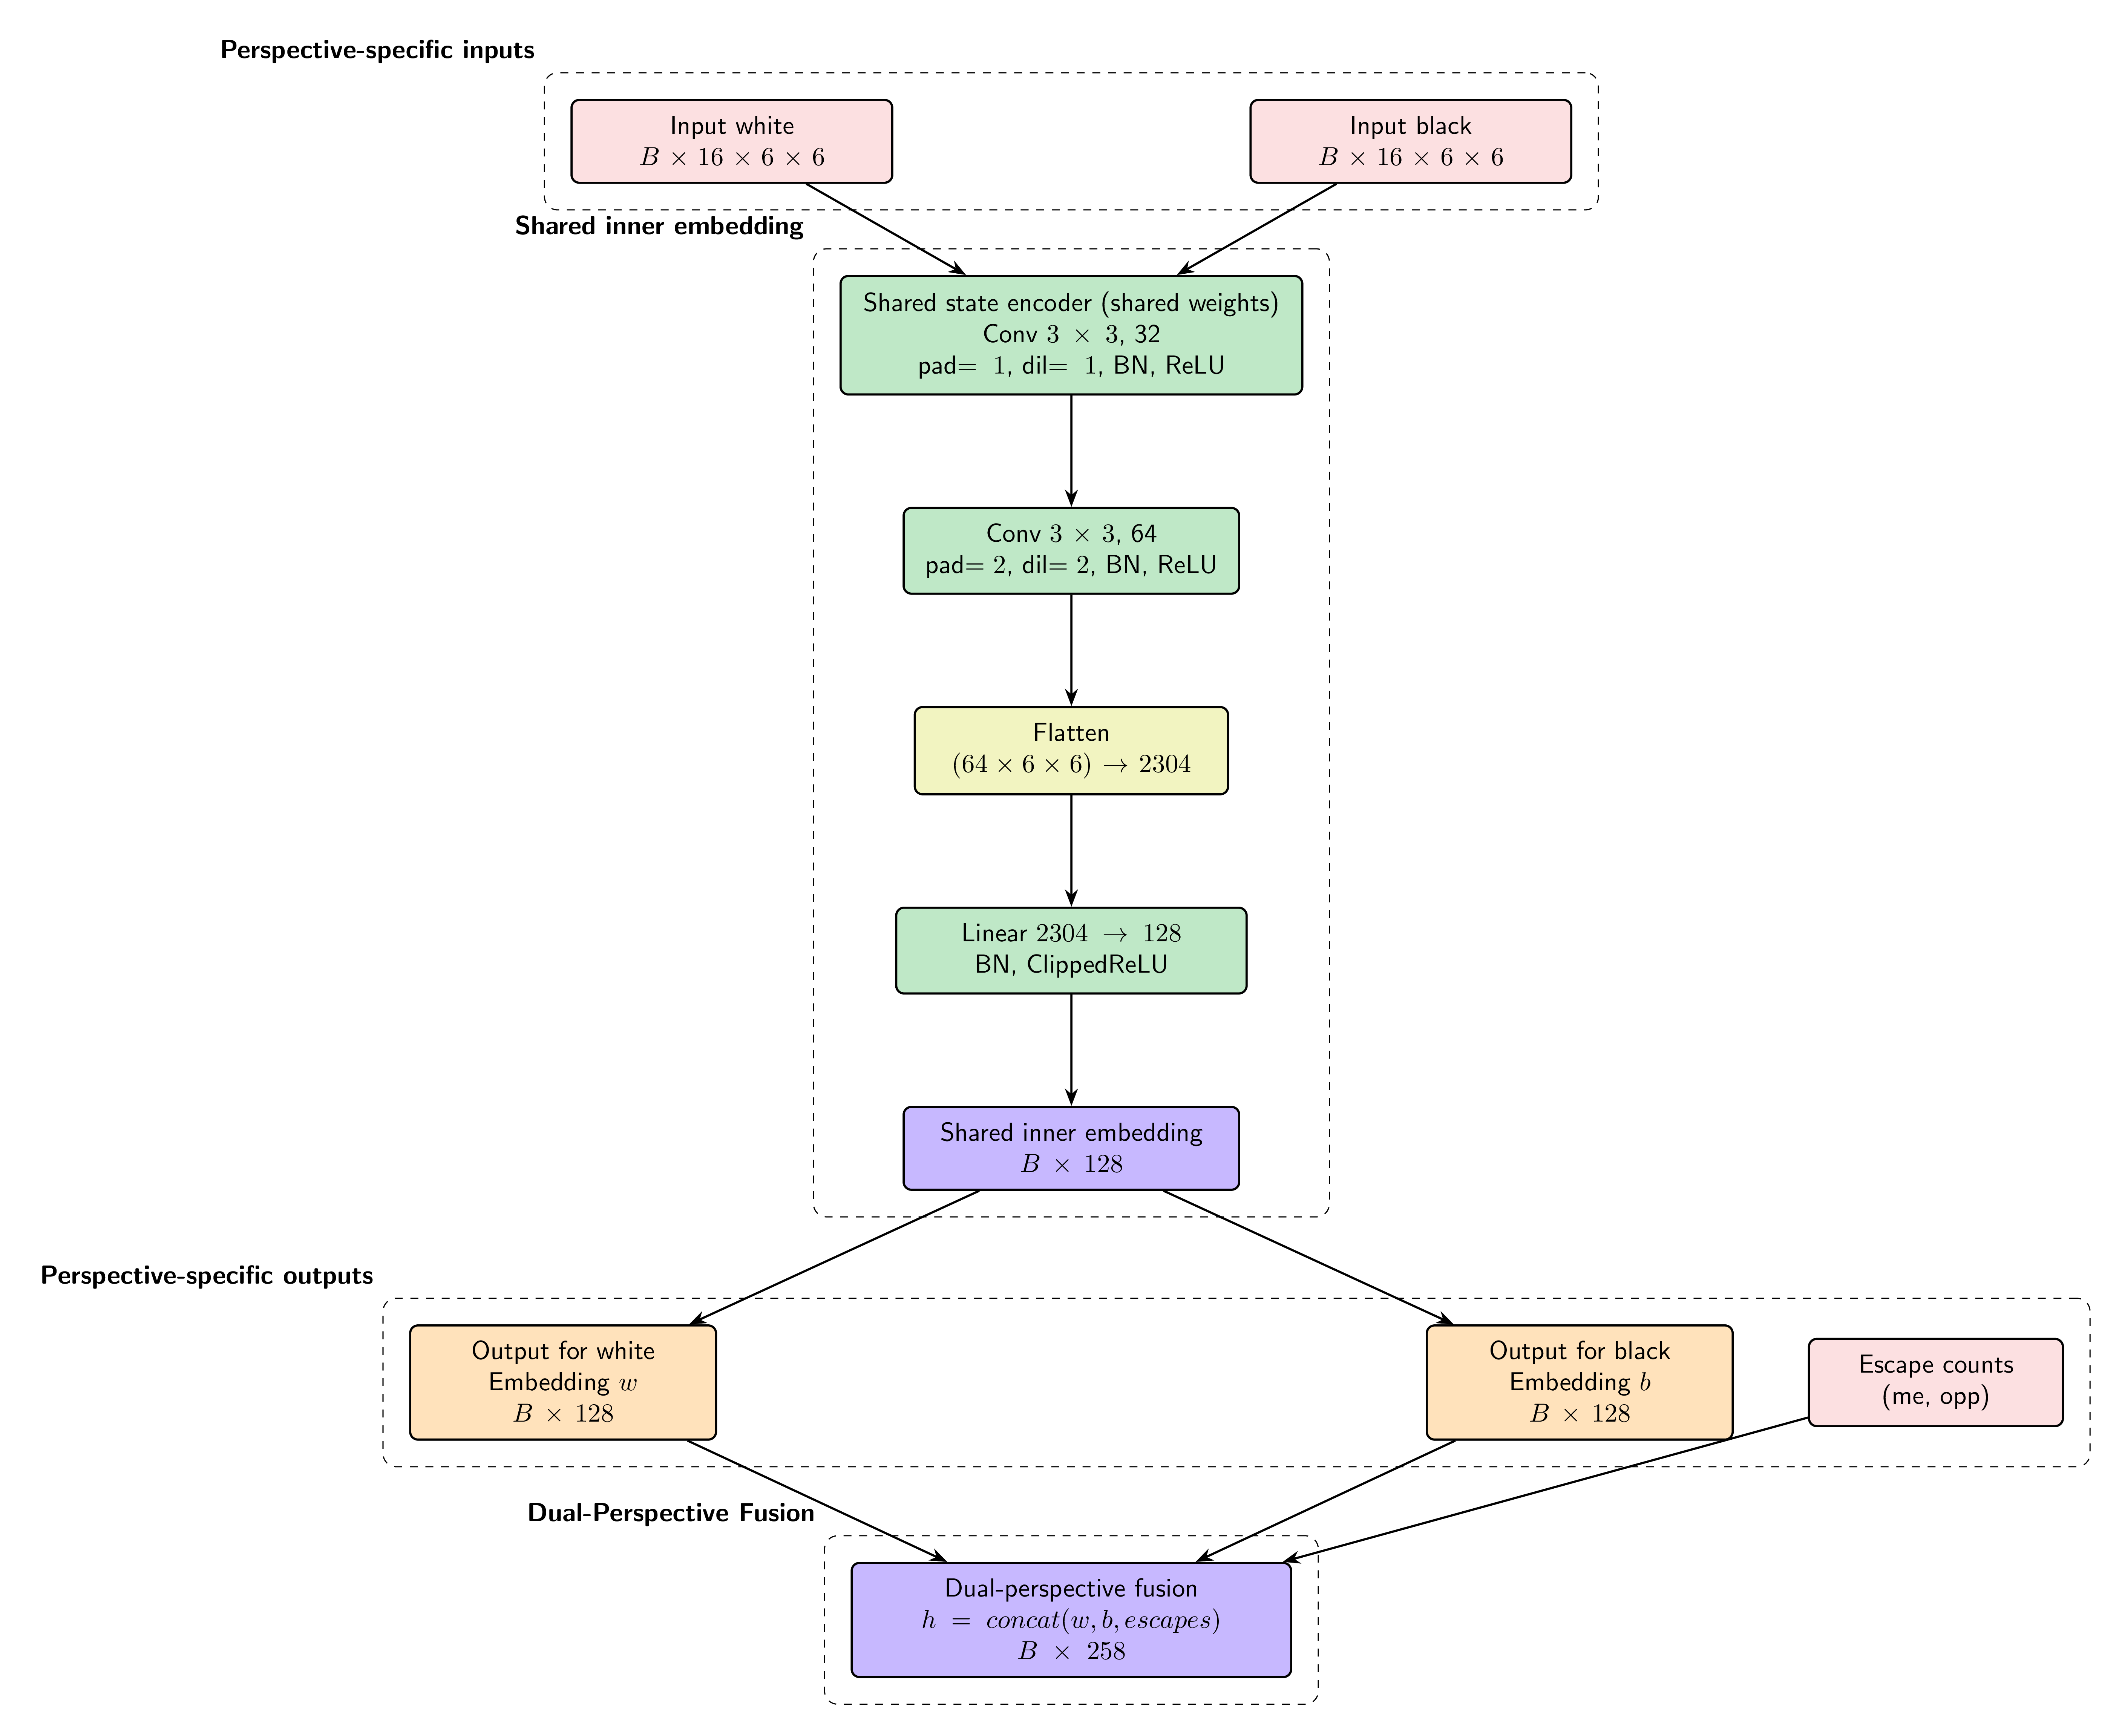
\includegraphics[width=0.85\textwidth]{model/components/SSE.png}
    \caption{Structure de l'encodeur spatial partagé (Shared Spatial Encoder) utilisé pour chaque perspective (poids partagés).}
    \label{fig-shared-spatial-encoder}
\end{figure}

\paragraph{Fusion et tronc résiduel.}
Les deux embeddings (256 dimensions) sont concaténés avec deux scalaires normalisés (le nombre de coups légaux de chaque licorne (échappatoire)) formant un vecteur de 258 dimensions. Ce vecteur traverse 3 \texttt{ResBlocks} de même dimension (Linear $\to$ Dropout(0.2) $\to$ BN $\to$ ReLU $\to$ Linear $\to$ BN, puis connexion résiduelle + ClippedReLU). Les 3 niveaux correspondent aux trois abstractions naturelles du jeu : proximité/licorne-relative, interaction de bandes/tempo, forçage/échappatoire.
\begin{figure}[H]
    \centering
    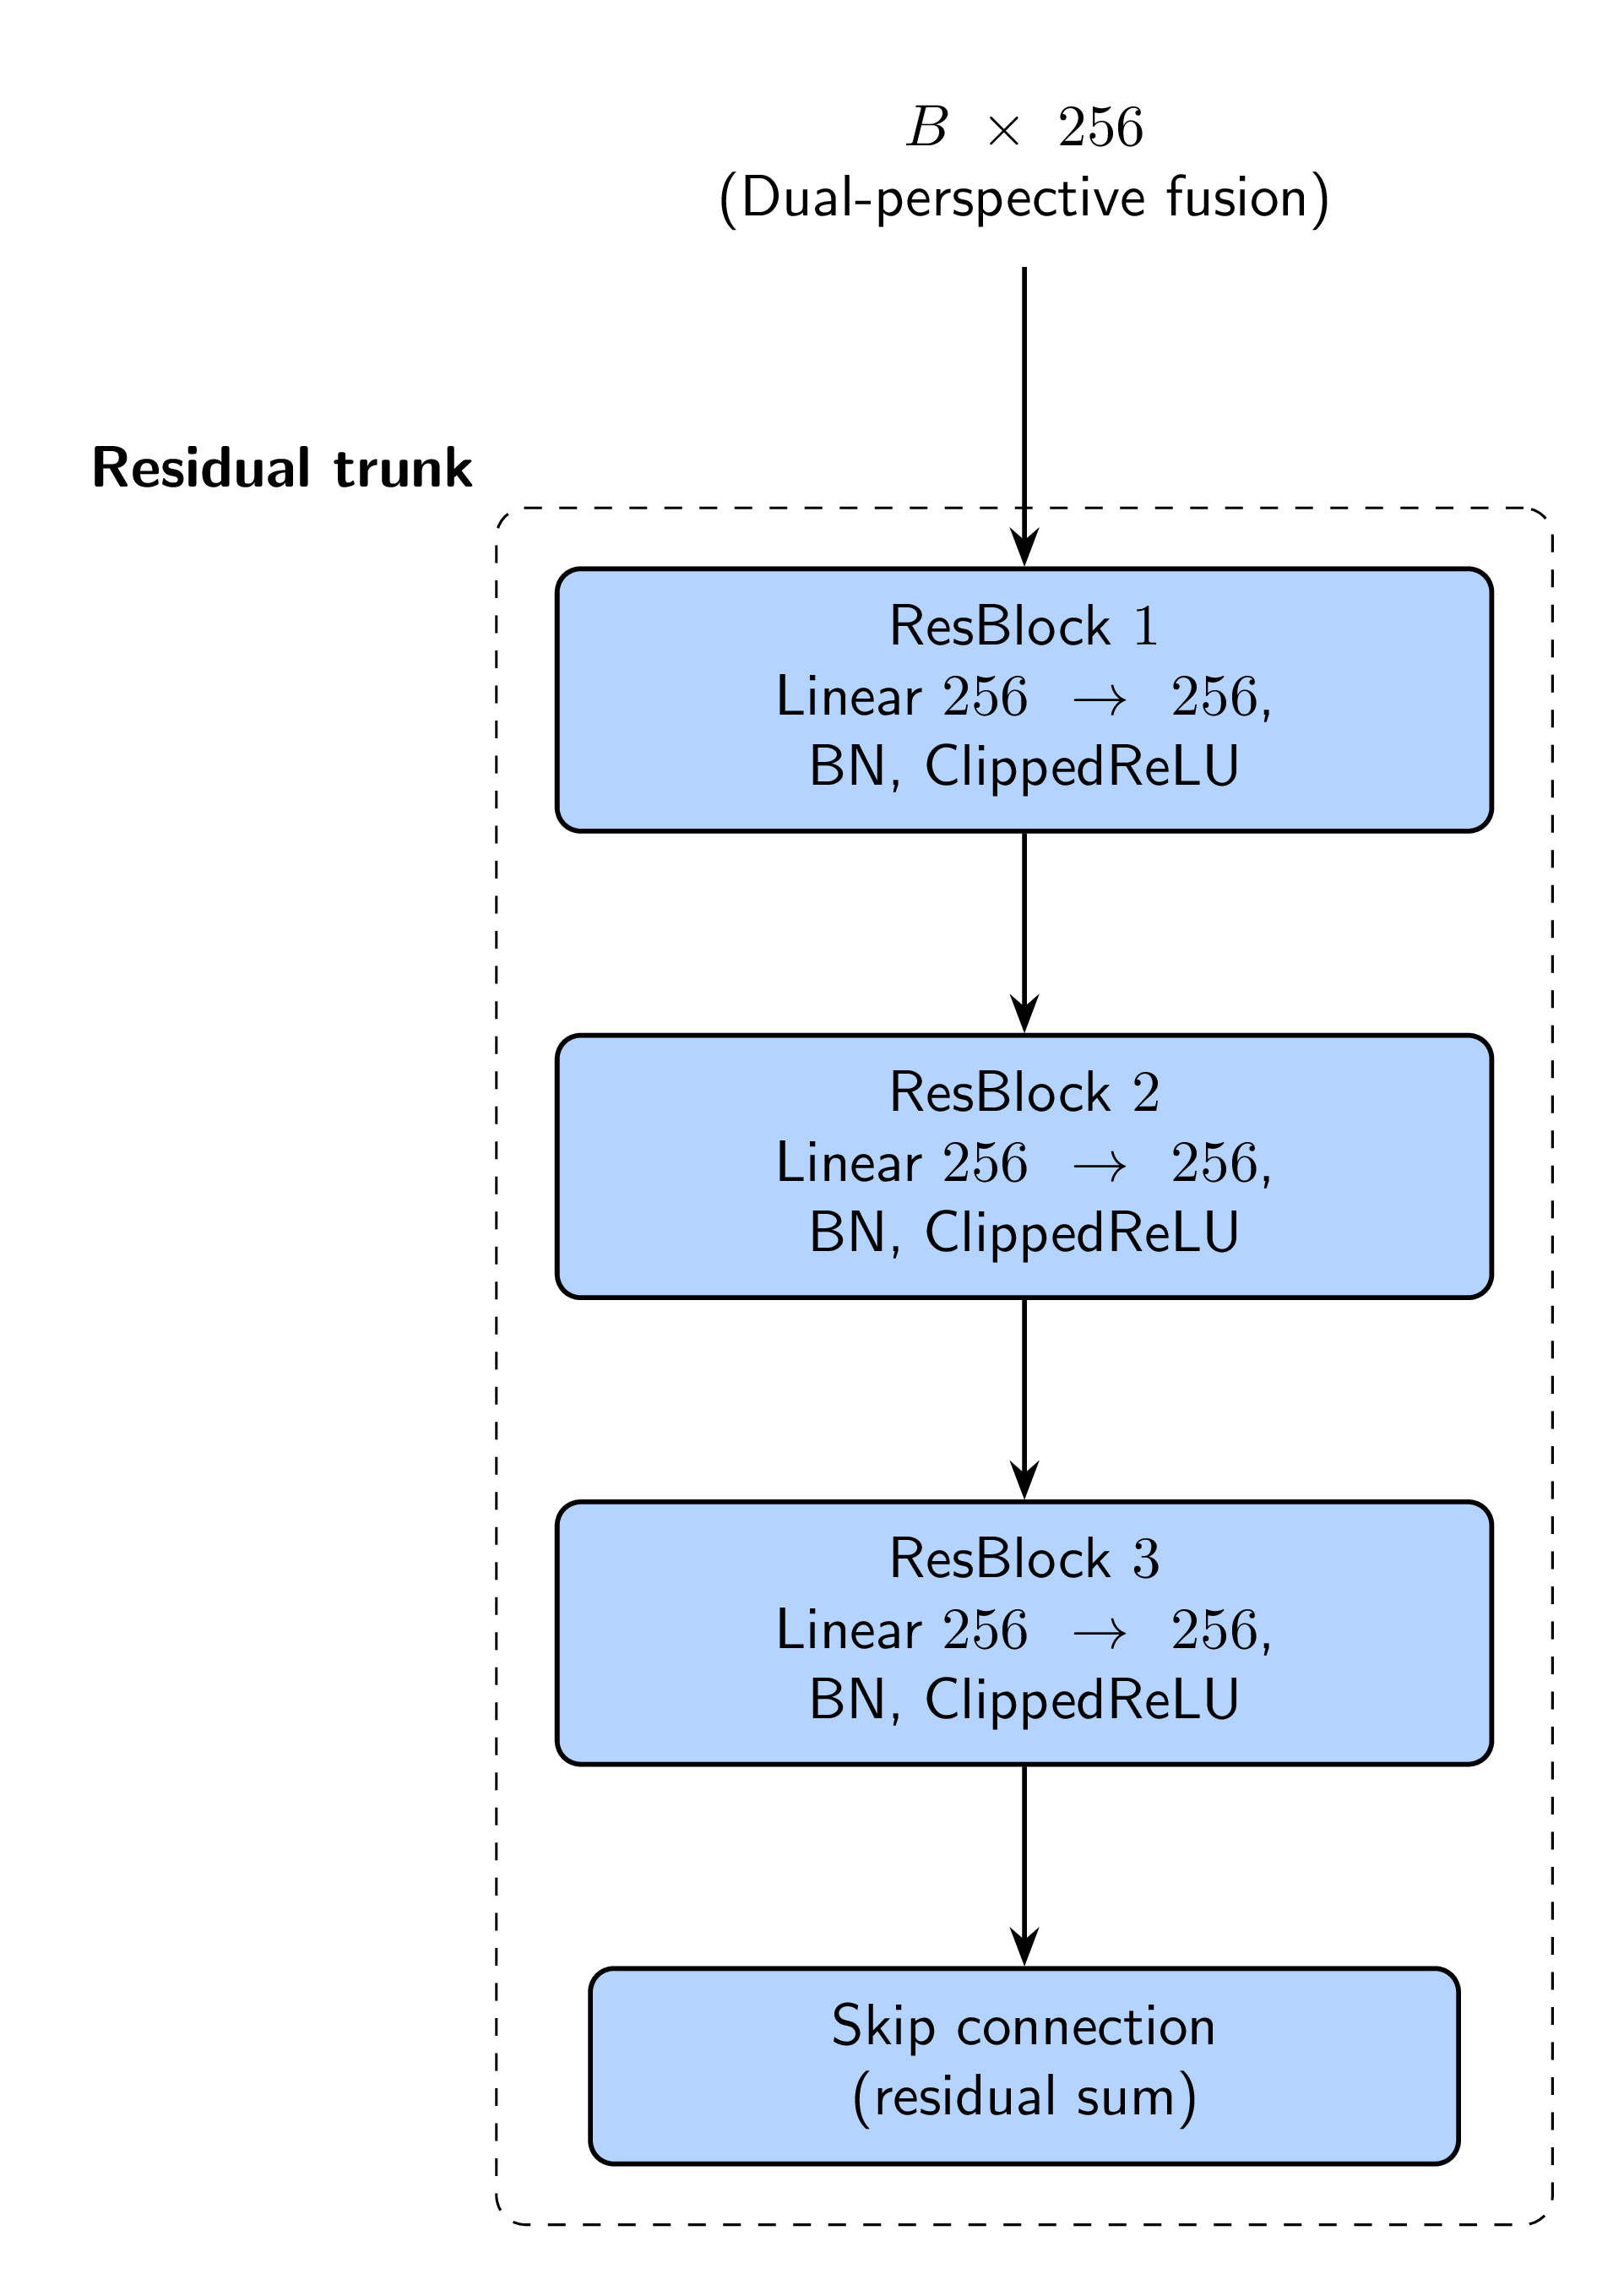
\includegraphics[width=0.7\textwidth]{model/components/residual_trunk.png}
    \caption{Structure du tronc résiduel avec blocs de correction résiduels (skip connections).}
    \label{fig-residual-trunk}
\end{figure}

\paragraph{Tête de sortie et raccourci.}
Linear$(258\to64)$ $\to$ ReLU $\to$ Linear$(64\to1)$ $\to$ $\tanh$, produisant un scalaire dans $[-1,+1]$. Un paramètre appris unique (\texttt{w\_forced\_pass}) s'additionne directement à la sortie brute sans traverser le tronc, inspiré du raccourci PSQT de Stockfish HalfKAv2~\cite{cp_nnue}. Ce bypass garantit un gradient fort pour les positions de passe forcée ($\sim$2--5\% du corpus), sans surcharger le tronc.

\begin{figure}[H]
    \centering
    
\includegraphics[width=0.7\textwidth]{model/components/output_head.png}
    \caption{Structure de la tête de sortie avec injection directe du signal de passe forcée (raccourci direct).}
    \label{fig-output-head}
\end{figure}


\paragraph{Bilan paramétrique.}
\begin{table}[H]
\centering
\begin{tabular}{p{7.5cm} p{2.5cm}}
\toprule
Composant & Paramètres \\
\midrule
Encodeur partagé (utilisé $\times 2$, poids identiques) & $\sim$312\,000 \\
Tronc résiduel (3 ResBlocks, dim=258) & $\sim$402\,648 \\
Tête de sortie & $\sim$16\,577 \\
\textbf{Total} & \textbf{$\sim$730\,625} \\
\bottomrule
\end{tabular}
\caption{Compte des paramètres par composant ($\approx$ 2,9 Mo en float32).}
\label{tab-parameter-count}
\end{table}

Une variante allégée (\texttt{embed\_dim=64}, 2 ResBlocks) atteint $\sim$185K paramètres pour une intégration plus rapide.


\subsection*{Génération des données et entraînement}
Les étiquettes sont générées par \textbf{amorçage Minimax} : pour chaque position échantillonnée en auto-jeu, un alpha-Beta à profondeur 4--6 calcule le score normalisé dans $[-1,+1]$. On vise 50K--100K positions labélisées. Les exemples stockent des triplets \texttt{(état, bande\_dernier\_coup, label)} pour conserver l'information de contrainte de bande et de passe forcée.
L'entraînement utilise une perte MSE, l'optimiseur AdamW ($\text{lr}=10^{-3}$, weight decay $10^{-4}$), un scheduler \textit{CosineAnnealingWarmRestarts} sur 40 époques (batch 256, split 90/10), et un \textit{gradient clipping} à 1,0. Les poids sont initialisés par Xavier uniforme (gain 0,5) pour éviter une saturation précoce des activations ClippedReLU.


\subsection*{Pipeline d'export et optimisations envisagées}
Pour l'intégration Java, BatchNorm est replié analytiquement dans les couches adjacentes avant l'export (éliminant les divisions au moment de l'inférence), puis les poids sont sérialisés en JSON ou exportés via ONNX Runtime (latence cible $\sim$1--2~$\mu$s pour le modèle \textbf{quantifié} en INT8 de 25\,K paramètres quantifiés).
Une \textbf{tête de politique} ajoutant une distribution sur les $\sim$96 coups légaux a été envisagée pour améliorer l'ordonnancement des coups à la racine.


\subsection*{Limites, ressources et statut d'intégration}
Nous avons pu générer plusieurs corpus de données:  
\begin{figure}[H]
    \centering
    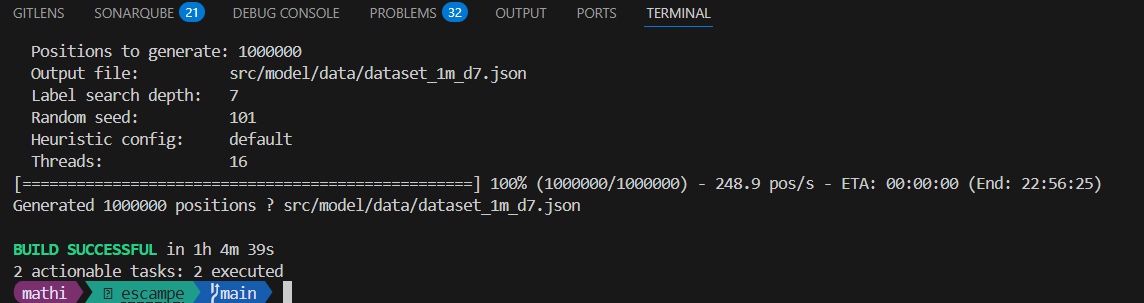
\includegraphics[width=0.7\textwidth]{images/data export 1m d7 parralel.png}
    \caption{Export de 1 million de parties à une profondeur de 7}
    \label{fig-data-export}
\end{figure}

Elles furent ensuite téléchargées sur \href{https://huggingface.co/datasets/Bluefir/escampe-dataset}{\textbf{Hugging Face}} pour l'entraînement du modèle BandDPER :  
\begin{figure}[H]
    \centering
    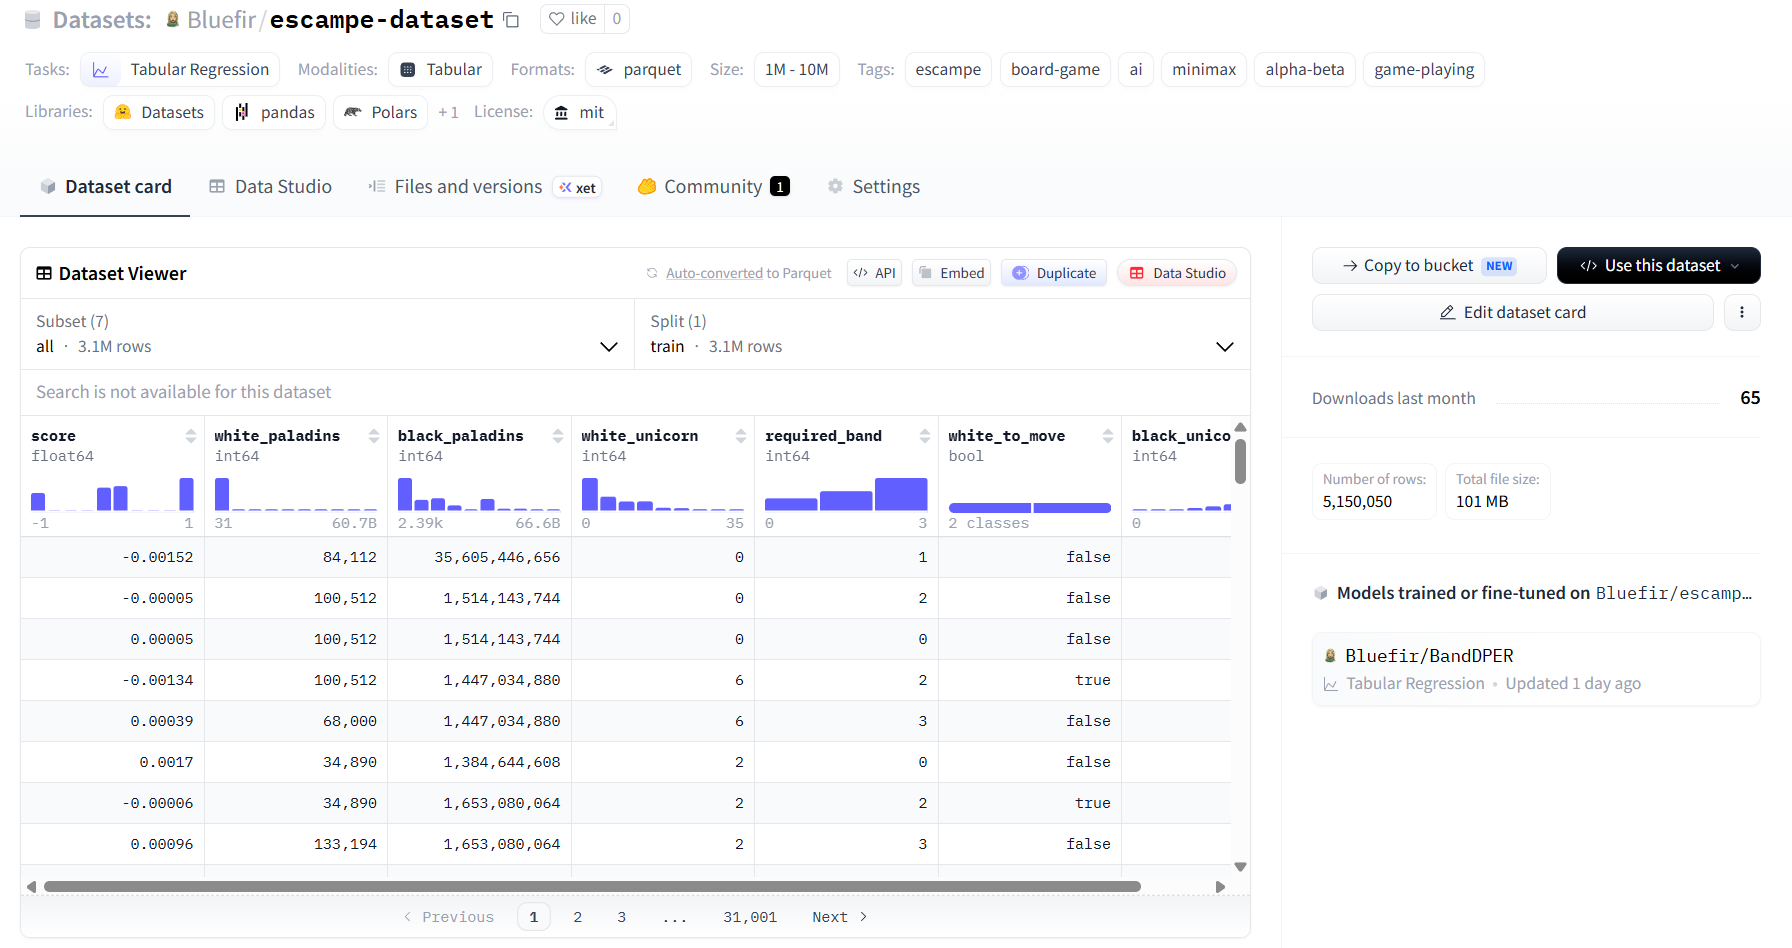
\includegraphics[width=0.7\textwidth]{images/hugggingface dataset.png}
    \caption{Dataset sur HuggingFace}
    \label{fig-dataset}
\end{figure}
Les colonnes d'entrée sont les suivantes :
\begin{itemize}
  \item \texttt{white\_paladins} : un entier long (bitboard) encodant la position des paladins blancs.
  \item \texttt{white\_unicorn} : l'indice de la case occupée par la licorne blanche (de 0 à 35). Logiquement, tend à être plus proche de 0 que de 35.
  \item \texttt{black\_paladins} : un entier long (bitboard) encodant la position des paladins noirs.
  \item \texttt{black\_unicorn} : l'indice de la case occupée par la licorne noire (de 0 à 35). Logiquement, tend à être plus proche de 35 que de 0.
  \item \texttt{required\_band} : le liseré/la bande imposé par le coup précédent (1, 2, 3 ou 0 si aucune contrainte).
  \item \texttt{white\_to\_move} : un booléen indiquant si c'est au joueur blanc de jouer.
  \item \texttt{score} : le score d'évaluation minimax obtenu à profondeur 5, normalisé entre $-1{,}0$ et $+1{,}0$ depuis la perspective du joueur actif.
\end{itemize}


En faisant un premier entraînement sur 50k positions, on obtient ce modèle (qui fait bien 2.9Mo):
\begin{figure}[H]
  \centering
  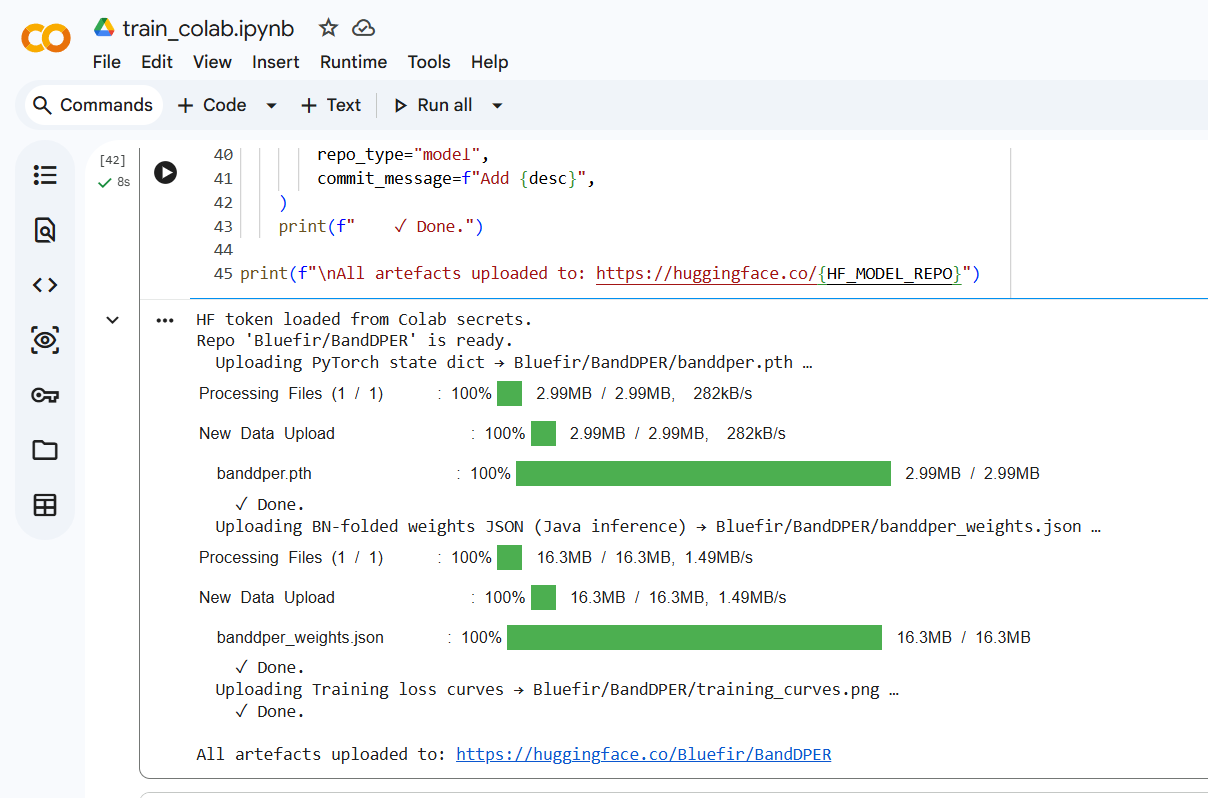
\includegraphics[width=0.7\textwidth]{images/model 50k.png}
    \caption{Entraînement initial sur 50k positions}
    \label{fig-model-50k}
\end{figure}

En revanche, on observe que le modèle overfit extrêmement :
\begin{figure}[H]
    \centering
    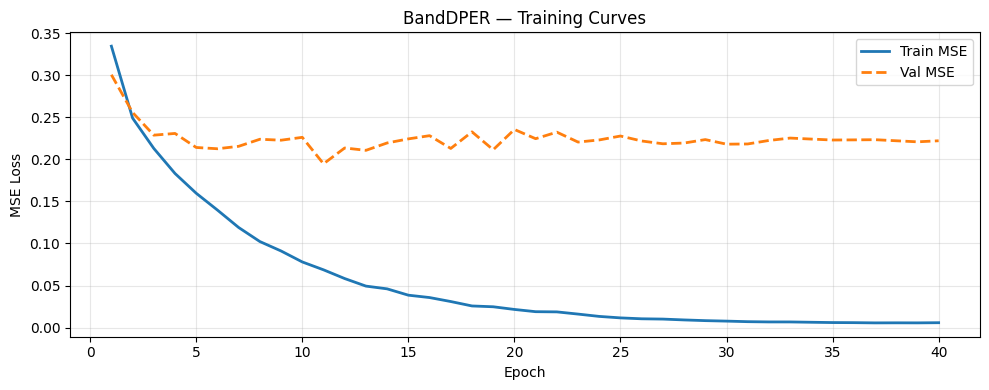
\includegraphics[width=0.7\textwidth]{images/model overfit 50k.png}
    \caption{Overfitting du modèle après entraînement initial}
    \label{fig-model-overfit-50k}
  \end{figure}

Le modèle a tout de même été exporté sur \href{https://huggingface.co/Bluefir/BandDPER}{\textbf{Hugging Face}}.
Pour régler le problème d'overfitting, nous avons mis à jour le modèle avec un dropout pour régulariser l'entraînement, et augmenté la taille du jeu de données à 3 millions de positions (6 millions en comptant les perspectives inversées).
Cependant, nous n'avons pas pu observer le résultat faute de temps d'entraînement suffisant :  
\begin{figure}[H]
    \centering
    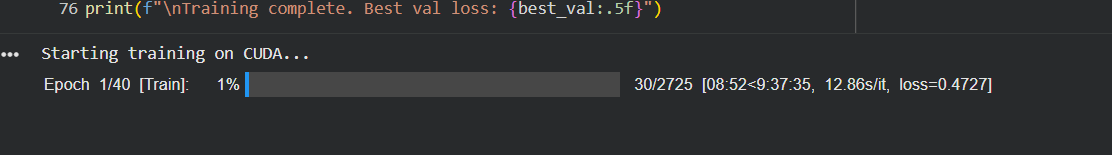
\includegraphics[width=0.7\textwidth]{images/model slow training.png}
    \caption{Entraînement sur 6 millions de positions avec dropout}
    \label{fig-model-6m}
\end{figure}


Pour plus d'informations techniques détaillées sur l'architecture, le processus d'entraînement et l'équivariance du modèle, veuillez consulter le document PDF dédié au modèle BandDPER (\texttt{model/BandDPER.pdf}).

BandDPER n'a pas été retenu comme heuristique principale : la latence d'inférence depuis Java reste incompatible avec les contraintes de temps par noeud de l'alpha-Beta profond. Son usage le plus prometteur reste l'ordonnancement à la racine (coût ponctuel, non répété), laissé comme piste de développement futur.






\section{Stratégie Initiale : Placement et Ouvertures}
\subsection{Principes de Placement (Opening Book)}
L'issue de la partie dépend grandement du positionnement initial. Contrairement aux Échecs, le plateau de départ d'Escampe est défini par les joueurs. Notre agent intègre une bibliothèque de placements de départ (\textit{Opening Book}) garantissant de solides propriétés structurelles :
\begin{itemize}
    \item \textbf{Couverture de toutes les bandes} : Les Paladins doivent couvrir idéalement les bandes 1, 2 et 3. Un déséquilibre offrirait à l'adversaire l'opportunité de cibler une bande où l'agent n'aurait aucune pièce, le contraignant à passer son tour immédiatement.
    \item \textbf{Dispersion sur les colonnes} : Éviter les grappes de Paladins qui se bloquent mutuellement. Nous essayons de placer au moins un paladin dans chaque colonne afin de conserver des lignes d'attaque ouvertes.
    \item \textbf{Sécurité de la Licorne} : Ne pas murer la Licorne avec ses propres pièces (ce qui l'empêcherait de s'enfuir), tout en s'assurant qu'elle ne soit pas exposée au centre. Les cases "double-bande" (ex: C1, F1, F2 en coordonnées relatives de départ) sont privilégiées pour leur équilibre entre mobilité d'évasion et protection naturelle.
\end{itemize}

Nous avons ainsi défini et implémenté huit configurations d'ouverture principales (pour le joueur Blanc, et leurs miroirs pour Noir) :
\begin{description}
    \item[\texttt{Balanced} (C1/A1/B2/D2/E2/F1)] : La licorne est placée sur la case ``double-bande'' centrale \texttt{C1}. Les paladins sont répartis sur toutes les colonnes et couvrent l'intégralité des 3 bandes (bande 1 sur F1, bande 2 sur E2, bande 3 sur A1, B2, D2).
    \item[\texttt{Widespread} (C1/A2/B1/D2/E1/F2)] : Les paladins sont dispersés de façon maximale sur les lignes 1 et 2 pour que le joueur conserve des options actives peu importe la contrainte imposée.
    \item[\texttt{Triple Dominance} (C1/A1/B2/D2/F2/E2)] : 5 paladins sur des cases de bande 3. Cette configuration maximise la portée et la mobilité d'agression dès le début de la partie.
    \item[\texttt{Central Pressure} (D1/A1/B2/C2/E2/F1)] : La licorne est placée en \texttt{D1} (bande 1, plus exposée) mais les paladins verrouillent le centre pour étouffer l'adversaire.
    \item[\texttt{Defensive} (B1/A2/C1/D2/E1/F2)] : La licorne est cachée dans un coin sécurisé (\texttt{B1}) et les paladins forment un bouclier sur la ligne 2.
    \item[\texttt{Flanking} (C1/D1/E1/A2/B2/F2)] : Concentration asymétrique des paladins sur un flanc pour forcer le passage par un couloir et menacer rapidement la licorne adverse.
    \item[\texttt{Defensive Edge} (A2/B1/C2/D1/E2/F2)] : La licorne est placée en \texttt{B1} avec une couverture avancée des paladins pour bloquer les attaques rapides à longue portée.
    \item[\texttt{Symmetric} (C1/A1/F1/B2/E2/D2)] : Une symétrie bilatérale parfaite autour de l'axe central du plateau pour équilibrer les capacités d'attaque sur les deux flancs.
\end{description}

En dehors de la phase de placement, l'agent met à profit les temps de réponse de l'arbitre grâce au \textbf{Pondering}~\cite{cp_pondering} : après avoir joué son coup, il prédit le meilleur coup adverse (100 ms de recherche rapide), applique ce coup hypothétique sur une copie du plateau, puis lance en arrière-plan un thread de recherche profonde (budget 4\,s). Si l'adversaire joue effectivement le coup prédit (\textit{ponder hit}), la réponse est déjà calculée et jouée instantanément, économisant du temps sur le budget principal. En cas d'échec (\textit{ponder miss}), le thread est interrompu et la recherche repart de zéro normalement.


\subsection{Stratégie par Phase de Jeu}
Une stratégie différenciée par phase peut améliorer significativement les performances :
\begin{description}
    \item[Début de partie] Placement équilibré couvrant plusieurs bandes (1, 2, 3). Licorne protégée derrière des paladins sans être enfermée. Éviter les couloirs directs vers sa licorne.
    \item[Milieu de partie] Jouer le tempo : choisir les cases d'arrivée pour imposer une mauvaise bande adverse ou forcer une passe. Créer des menaces doubles sur la licorne tout en maintenant une défense active. Limiter les coups qui offrent une bande favorable à l'adversaire.
    \item[Fin de partie] Chercher les séquences forçantes (capture en 1--3 coups) via une recherche plus profonde grâce à l'approfondissement itératif et à la réduction du budget temporel. En défense, maximiser la mobilité de la licorne et casser les lignes d'attaque.
\end{description}






\section{Gestion du Temps Réel}
\label{sec-time}
La communication avec le serveur impose des temps limites stricts sous peine de défaite immédiate. Nous avons implémenté un \texttt{TimeManager}~\cite{cp_time} hybride avec gestion dynamique des bornes.

\begin{itemize}
    \item \textbf{Estimation du temps par coup} : Le temps de base alloué est calculé en divisant le temps global restant par une estimation dynamique du nombre de coups restants. Cette estimation s'adapte selon la réserve : 40 coups supposés s'il reste beaucoup de temps ($> 200$~s), puis descend par paliers (25, 15) jusqu'à 8 coups en fin de partie critique.
    \item \textbf{Facteur de Complexité} : Un multiplicateur ajuste le budget temporel en fonction du nombre de coups légaux. Si le joueur n'a qu'un ou deux coups quasi-forcés (contrainte de bande), le budget est drastiquement réduit (facteur de 0,3) pour économiser du temps. Dans une position très ouverte ($\ge 20$ coups), le budget augmente (facteur 1,5).
    \item \textbf{Soft Bound / Hard Bound} : 
    \begin{itemize}
        \item La \textit{Soft Bound} (limite logicielle) correspond au budget temporel de base ajusté. Une fois franchie, la boucle d'\textit{Iterative Deepening} s'interrompt pour renvoyer le meilleur coup de la dernière profondeur complète.
        \item La \textit{Hard Bound} (limite matérielle) agit comme une sécurité absolue, fixée à $3 \times$ la \textit{Soft Bound} (avec un plafond strict à un cinquième du temps total restant). Si elle est atteinte en plein milieu de l'évaluation d'un noeud (lors des appels récursifs du Minimax), l'algorithme coupe instantanément la branche et retourne l'évaluation heuristique courante, empêchant ainsi le dépassement de temps fatal.
    \end{itemize}
\end{itemize}





\section{Analyse des Performances et Tests}
Les performances de l'IA ont été évaluées via un moteur de test autonome opposant plusieurs versions de notre agent.


\subsection{Évaluation Elo et Test SPRT}
L'amélioration des heuristiques et l'optimisation des structures de données ont été quantifiées via un système de tournoi automatique (\texttt{TournamentRunner}) opposant de multiples configurations de notre agent. Le classement repose sur le rating Elo avec mise à jour $R' = R + K(S - E)$, où $E = 1/(1 + 10^{(R_B - R_A)/400})$ et $K = 32$. Les configurations testées incluent différentes profondeurs (2 à 6), les deux algorithmes de recherche (AlphaBetaKH et NegamaxKH), les trois variants d'heuristique (Default, SimplexFull, BandCoverage-ablated) et l'activation ou non du Pondering.

Pour valider statistiquement qu'une modification apporte un gain Elo réel avant de la valider, nous utilisons le \textbf{SPRT}~\cite{cp_testing} (\textit{Sequential Probability Ratio Test}). Le SPRT compare deux hypothèses : $H_0$ (les deux agents sont équivalents, Elo $= 0$) contre $H_1$ (l'un est meilleur, Elo $> 0$). Le test s'arrête dès que les données accumulées sont suffisantes pour accepter ou rejeter $H_0$ au seuil de confiance fixé (95\%), évitant de jouer des parties inutiles. Ce processus itératif, inspiré des pratiques de Stockfish, garantit que seules les améliorations réelles progressent vers la version finale.
\begin{figure}[H]
    \centering
    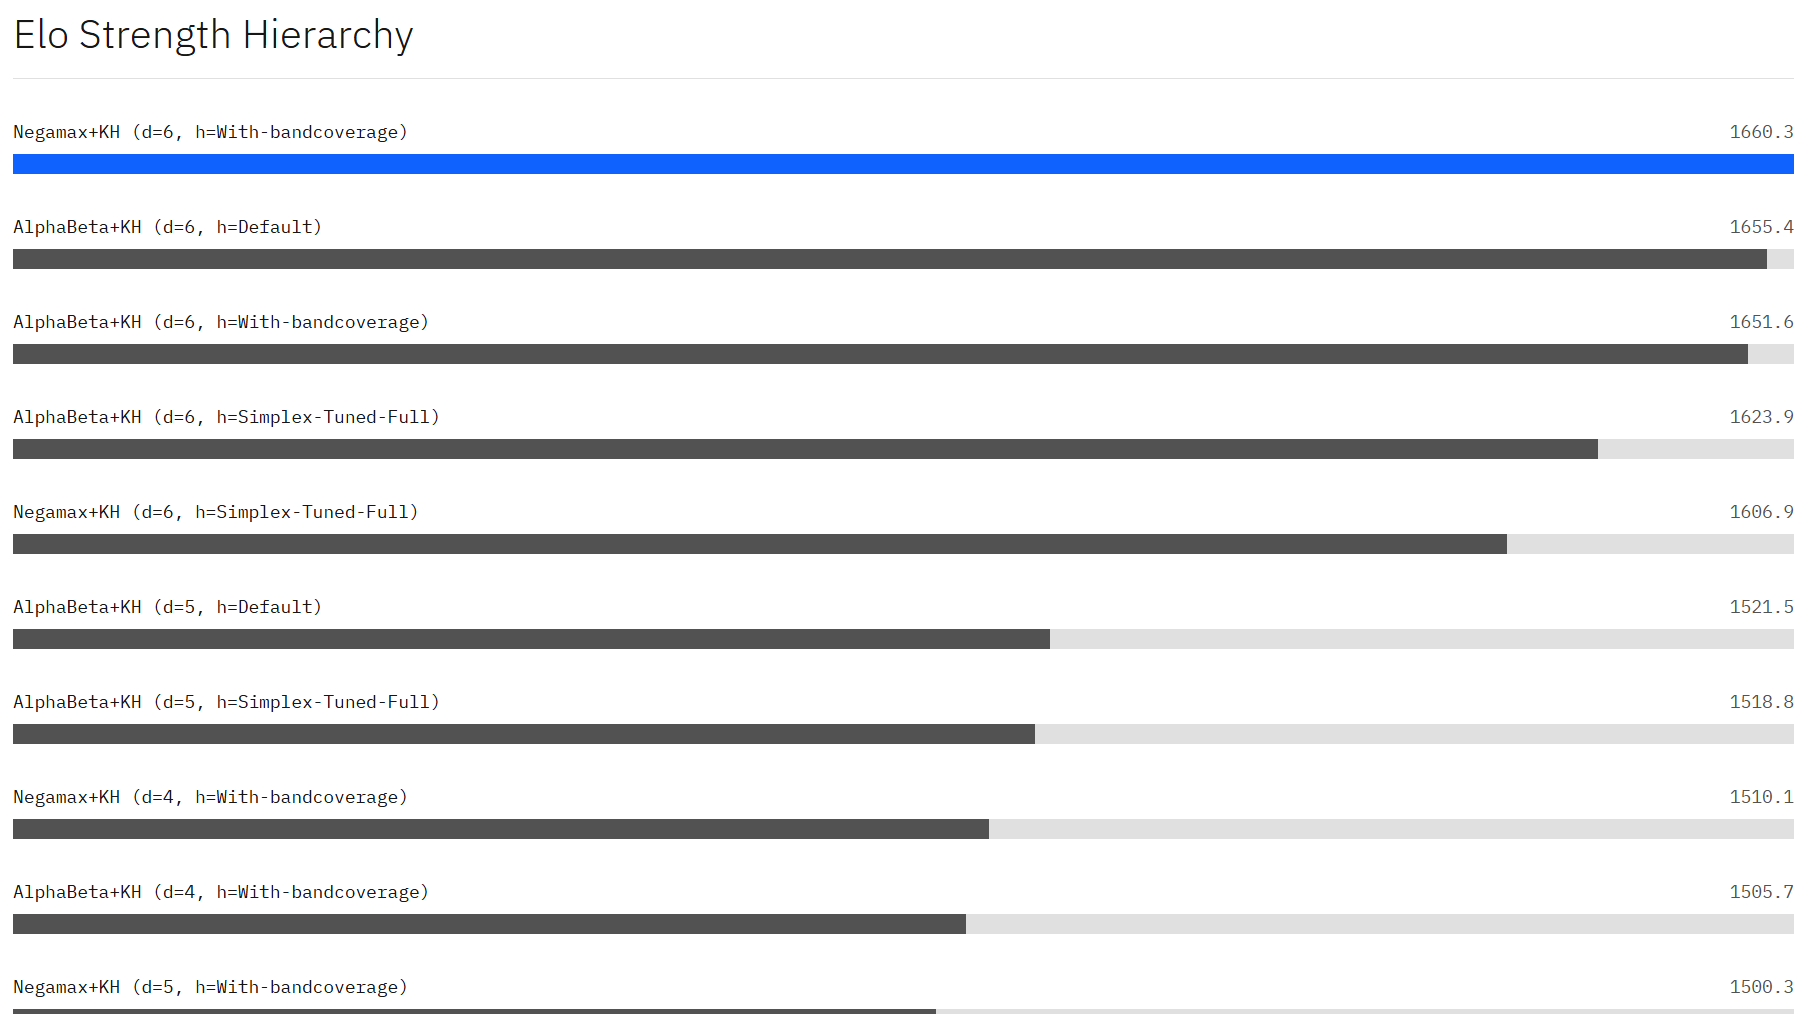
\includegraphics[width=0.7\textwidth]{images/ranking.png}
    \caption{Évolution du classement Elo des différentes configurations testées (tests SPRT) sur 2000 parties par matchup.}
    \label{fig-elo-ranking}
\end{figure}
Le test n'est significatif que lorsque le nombre de parties jouées dépasse un certain seuil (généralement plusieurs centaines ou milliers) pour réduire l'impact de la variance. 
A noter aussi que certaines améliorations sont invisibles à faible profondeur (ex: ordonnancement des coups) et ne montrent leur plein potentiel qu'à partir de la profondeur 4 ou 5, d'où l'importance de tester sur plusieurs profondeurs.
Voici le premier test réalisé:  
\begin{figure}[H]
    \centering
    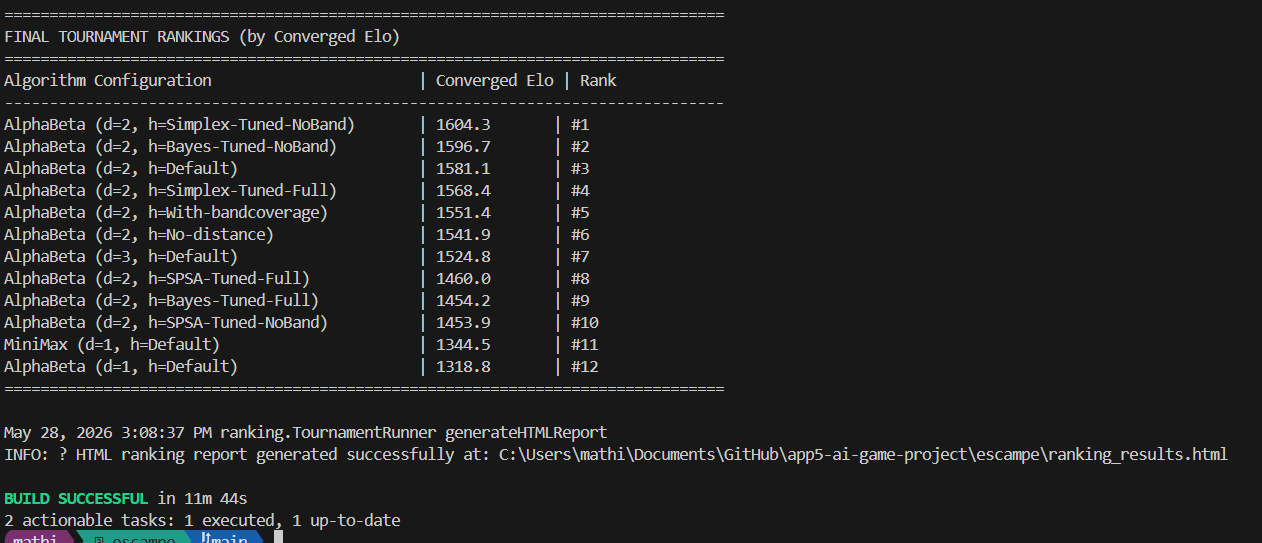
\includegraphics[width=0.7\textwidth]{images/first ranking with tuning.png}
    \caption{Premier test de classement Elo après implémentation des fonctionnalités principales et heuristiques calibrées.}
    \label{fig-sprt-test}
\end{figure}


\subsection{Validation de la Conduite Autonome}
Les protocoles de communication avec l'arbitre ont été validés localement en s'assurant qu'aucun dépassement de délai n'intervenait et que tous les coups générés restaient strictement conformes aux règles topologiques du jeu.





\section{Bilan des Fonctionnalités et Statut du TODO}
\label{sec-todo-status}
Afin de mesurer le travail accompli au cours du projet et de structurer les développements futurs, un suivi rigoureux a été maintenu sous la forme d'un tableau d'objectifs (TODO). Cette section dresse le bilan des fonctionnalités implémentées, validées et de celles envisagées comme perspectives d'amélioration.


\subsection{Fonctionnalités Entièrement Implémentées et Validées}
\begin{itemize}
    \item \textbf{Moteur de Recherche et Pruning} : Implémentation complète de l'algorithme \texttt{Negamax} avec élagage Alpha-Beta symétrique. L'approfondissement itératif (\textit{Iterative Deepening}) a été déployé avec succès, garantissant une flexibilité absolue face aux limites de temps de réflexion.
    \item \textbf{Gestion Fine du Temps} : Mise en oeuvre du \texttt{TimeManager} avec un double niveau de sécurité (\textit{Soft Bound} pour clore proprement la recherche à la fin d'une profondeur donnée, et \textit{Hard Bound} coupant instantanément l'exécution récursive du minimax en cas d'urgence). Le temps est mesuré à haute résolution via \texttt{System.nanoTime()}.
    \item \textbf{Ordonnancement des Coups} : Intégration d'un ordonnanceur de coups (\texttt{MoveOrderer}) combinant l'heuristique des coups tueurs (\textit{Killer Heuristic} avec FIFO à 2 slots) et l'heuristique de l'historique (\textit{History Heuristic} pondérée par la profondeur au carré). Le tri est réalisé \textit{in-place} pour minimiser l'impact mémoire.
    \item \textbf{Heuristiques Linéaires Calibrées} : Conception d'une formule d'évaluation combinant la proximité d'attaque, la proximité de défense, la mobilité/escapabilité de la licorne, le contrôle de bande et la pression de tempo. Ces poids ont été calibrés par optimisation stochastique SPSA. L'analyse d'ablation a conduit à exclure le terme de contrôle des bandes pour de meilleures performances (variant \texttt{BandCoverage-ablated}).
    \item \textbf{Bibliothèque d'Ouvertures et Réflexion en Temps Masqué} : Intégration d'un livre d'ouvertures diversifié (Balanced, Central Pressure, Symmetric, Flanking, etc.) assurant une bonne couverture de départ. Déploiement du mécanisme de \textit{Pondering} via un thread d'arrière-plan analysant le coup adverse supposé pendant son temps de réflexion (avec gestion des cas de \textit{ponder hit} et \textit{ponder miss}).
    \item \textbf{Optimisations Système et Représentation} : Passage d'une représentation matricielle classique à des Bitboards (\texttt{long} de 64 bits en Java), élimination des vérifications \texttt{instanceof} et implémentation du mécanisme \textit{Make-Unmake} pour éviter le clonage d'objets et stabiliser le Garbage Collector.
    \item \textbf{Conception du Modèle de Deep Learning} : Modélisation, génération de données (Minimax bootstrapping à profondeur 5, 50K-100K positions), entraînement sous PyTorch du modèle BandDPER, et intégration des mécanismes d'export (repliement analytique de BatchNorm).
\end{itemize}


\subsection{Fonctionnalités Conçues, Rejetées ou Non Retenues}
\begin{itemize}
    \item \textbf{Contrôle de Bande dans l'Heuristique} : Bien que central dans les règles du jeu, le contrôle manuel des bandes a été rejeté après tests SPRT et ablation, car il nuisait statistiquement au classement Elo global de l'agent.
    \item \textbf{Utilisation Directe du Réseau de Neurones en Jeu} : Le réseau BandDPER n'a pas été retenu comme fonction d'évaluation principale dans l'arbre en raison de sa latence d'évaluation trop élevée par rapport à l'heuristique linéaire optimisée en Java. Il est en revanche préconisé pour l'ordonnancement à la racine.
\end{itemize}


\subsection{Perspectives et Travaux Futurs (TODO Ouverts)}
\begin{itemize}
    \item \textbf{Table de Transposition et Zobrist Hashing} : Le schéma d'encodage par hachage Zobrist a été conçu mais n'a pas été finalisé dans l'exécution principale. Son intégration permettrait de stocker les scores d'évaluation des noeuds déjà parcourus et d'identifier instantanément les répétitions de positions (détection de boucles de jeu).
    \item \textbf{Élagages Sélectifs Avancés} : Intégration de techniques d'élagage plus agressives comme le \textit{Null-Move Pruning} (pour éliminer rapidement les branches très favorables), le \textit{Late Move Reduction} (LMR) pour réduire la profondeur d'exploration des coups moins prometteurs, et la recherche de quiescence (\textit{Quiescence Search}) aux feuilles.
    \item \textbf{Aspiration Windows} : Utilisation de fenêtres de recherche resserrées au lieu d'une fenêtre de recherche infinie lors de l'approfondissement itératif, pour maximiser l'élagage lorsque l'évaluation est stable.
    \item \textbf{Inférence ONNX Quantifiée} : Intégration finale de l'exécuteur ONNX Runtime pour charger le modèle BandDPER quantifié en INT8 et l'évaluer en temps réel sous une latence ciblée de 1 à 2 $\mu$s par coup.
\end{itemize}





\section{Conclusion et Difficultés Rencontrées}
La conception et la mise au point de cette Intelligence Artificielle pour le jeu d'Escampe ont constitué un défi d'ingénierie et d'algorithmique particulièrement stimulant. Au-delà des théories classiques sur la programmation des jeux de plateau, la nature hautement asymétrique et contrainte de l'Escampe a soulevé plusieurs catégories de difficultés majeures que nous avons dû surmonter :

\begin{enumerate}
    \item \textbf{Modélisation de la Topologie et Séquences Tactiques (Bandes)} : 
    Le plateau d'Escampe se distingue par une absence d'uniformité géométrique en raison de la répartition asymétrique des bandes (liserés 1, 2 et 3). Cette caractéristique brise toute propriété d'équivariance par translation spatiale simple, rendant les représentations classiques (comme les grilles d'occupation convolutionnelles pures) insuffisantes pour capturer les relations de menace. De plus, l'absence de capture progressive de pièces (la seule capture étant celle de la Licorne en fin de partie) allonge considérablement la longueur des séquences tactiques et empêche toute simplification rapide du jeu, exacerbant les effets d'horizon de la recherche minimax.
    
    \item \textbf{Complexité du Débogage de la Recherche sous Contraintes Temporelles} :
    L'intégration conjointe de l'élagage Alpha-Beta avec l'approfondissement itératif, l'ordonnancement dynamique des coups (Killer Heuristic à 2 slots et History Heuristic) et les coupures asynchrones (\textit{Soft} et \textit{Hard bounds} gérées par threads) a été une source de bogues subtils. Le choix d'une architecture \textit{Make-Unmake} pour éviter le Garbage Collector imposait de restaurer l'état exact du plateau après chaque évaluation récursive. En cas d'interruption abrupte (sécurité matérielle \textit{Hard Bound} franchie au milieu de la boucle minimax), la moindre désynchronisation sur les bitboards entraînait des états de jeu corrompus sur les noeuds frères suivants.
    
    \item \textbf{Optimisation dans un Espace de Poids Fortement Non-linéaire} :
    L'influence des paramètres de notre fonction d'évaluation manuelle était complexe à évaluer intuitivement. Par exemple, l'ablation et le calibrage stochastique SPSA ont contredit notre intuition initiale concernant l'importance du terme de contrôle des bandes pour notre propre joueur : la pénalisation trop forte des bandes manquantes restreignait excessivement le dynamisme offensif de notre IA, alors que la maximisation du piège adverse sur les bandes restrictives restait cruciale. La descente de gradient SPSA parallèle et le test d'hypothèse séquentiel (SPRT Elo) ont été indispensables pour prouver scientifiquement l'efficacité de nos réglages.
    
    \item \textbf{Arbitrage entre Puissance d'Évaluation et Latence d'Inférence (Deep Learning)} :
    La mise en oeuvre du modèle de Deep Learning \textbf{BandDPER} sous PyTorch et son export Java ont révélé le compromis inhérent aux IA de jeu modernes. Bien que le réseau de neurones résiduel siamois soit bien plus qualitatif pour appréhender les menaces positionnelles non-linéaires par rapport à notre heuristique linéaire de Manhattan, la latence d'inférence (de l'ordre de 1 à 2 $\mu$s par position avec ONNX Runtime quantifié en INT8) s'est avérée prohibitive par rapport à l'évaluation en pure logique Java (qui s'exécute en quelques nanosecondes). C'est pourquoi nous avons rejeté BandDPER comme fonction d'évaluation aux feuilles de l'arbre, limitant son potentiel d'intégration futur à un rôle d'ordonnanceur à la racine.
\end{enumerate}

En définitive, ce projet démontre qu'une IA performante repose autant sur l'efficacité brute de ses structures de données (Bitboards hybrides, Make-Unmake) et de sa recherche (ordonnancement, iterative deepening) que sur la rigueur de sa méthodologie de validation de performances (Elo local, SPRT, SPSA). Les pistes de développement futur (Zobrist hashing et tables de transposition complètes) devraient permettre de repousser encore les limites de profondeur atteintes par notre agent.




% ── Bibliographie ──────────────────────────────────────────────────────────────
\newpage
\begin{thebibliography}{9}

\bibitem{shannon1950}
C. E. Shannon,
\textit{Programming a computer for playing chess},
Philosophical Magazine, Ser. 7, 41(314), 256--275, 1950.
\url{https://doi.org/10.1080/14786445008521796}

\bibitem{knuth1975}
D. E. Knuth and R. W. Moore,
\textit{An analysis of alpha-beta pruning},
Artificial Intelligence, 6(4), 293--326, 1975.
\url{https://doi.org/10.1016/0004-3702(75)90019-3}

\bibitem{spall1998}
J. C. Spall,
\textit{An overview of the simultaneous perturbation stochastic approximation (SPSA) method},
Johns Hopkins APL Technical Digest, 19(4), 482--492, 1998.
\url{https://www.jhuapl.edu/Content/techdigest/pdf/V19-N04/19-04-Spall.pdf}

\bibitem{cp_alphabeta}
Chess Programming Wiki,
\textit{Alpha-Beta},
\url{https://www.chessprogramming.org/Alpha-Beta}

\bibitem{cp_bitboards}
Chess Programming Wiki,
\textit{Bitboards},
\url{https://www.chessprogramming.org/Bitboards}

\bibitem{cp_iterative_deepening}
Chess Programming Wiki,
\textit{Iterative Deepening},
\url{https://www.chessprogramming.org/Iterative_Deepening}

\bibitem{cp_time}
Chess Programming Wiki,
\textit{Time Management},
\url{https://www.chessprogramming.org/Time_Management}

\bibitem{cp_pondering}
Chess Programming Wiki,
\textit{Pondering},
\url{https://www.chessprogramming.org/Pondering}

\bibitem{cp_move_ordering}
Chess Programming Wiki,
\textit{Move Ordering},
\url{https://www.chessprogramming.org/Move_Ordering}

\bibitem{cp_killer}
Chess Programming Wiki,
\textit{Killer Heuristic},
\url{https://www.chessprogramming.org/Killer_Heuristic}

\bibitem{cp_nullmove}
Chess Programming Wiki,
\textit{Null Move Pruning},
\url{https://www.chessprogramming.org/Null_Move_Pruning}

\bibitem{cp_lmr}
Chess Programming Wiki,
\textit{Late Move Reductions},
\url{https://www.chessprogramming.org/Late_Move_Reductions}

\bibitem{cp_zobrist}
Chess Programming Wiki,
\textit{Zobrist Hashing},
\url{https://www.chessprogramming.org/Zobrist_Hashing}

\bibitem{cp_testing}
Chess Programming Wiki,
\textit{Match Statistics (SPRT)},
\url{https://www.chessprogramming.org/Match_Statistics}

\bibitem{cp_nnue}
Yu Nasu, \textit{Efficiently Updatable Neural-Network-based Evaluation Functions for Computer Shogi},
The 28th World Computer Shogi Championship Appeal Document, 2018.
\url{https://official-stockfish.github.io/docs/nnue-pytorch-wiki/docs/nnue.html}

\bibitem{bromley1993}
J. Bromley et al.,
\textit{Signature Verification using a Siamese Time Delay Neural Network},
NeurIPS, 1993.
\url{https://papers.nips.cc/paper/1993/hash/0d4262ad58b4d3866d5aa0f4f9e1c06b-Abstract.html}

\bibitem{alphazero}
D. Silver et al.,
\textit{Mastering Chess and Shogi by Self-Play with a General Reinforcement Learning Algorithm},
arXiv:1712.01815, 2017.
\url{https://arxiv.org/abs/1712.01815}

\end{thebibliography}

\end{document}